\begin{savequote}[75mm]
To forecast you need to know. 
\qauthor{Fabrizio Serafini}
\end{savequote}

\chapter{Introduction}
\section{Motivation}
 Can data play a central role in enhancing our understanding of global emissions and allowing us to make strategic decisions when decarbonizing? Can we build a more sustainable future by focusing on what matters the most and by making better use of the data we have? What other data do we need to make better decisions? Can we predict future decarbonization rates and, if so, what is the best way to do it? Those are only a few of the very important and interesting questions that drew me to research decarbonization and to focus on the role of corporate emission-level data in the process. I believe that the answers to those questions are crucial to our ability to build a more sustainable future and that the role of data in the process is central. Furthermore, those questions play a central role not only in a social and environmental perspective, but also in a business perspective. Indeed, the answers to those questions can help us make better decisions and, as a result, can help us build a more sustainable future while also creating value for businesses. Additionally, the call for more data in decarbonization comes not only from the academic world but also from the fact that many business opportunities arise from the climate transition that inevitably requrie good and valid information to determine which companies and sectors are winners and loosers, which are the champions in the decarbonization process, which are the laggards, and which are the companies that are greenwashing. I believe that studying specifically corporate emissions and forecasting decarbonization rates as I am doing in this thesis can be useful to three key stakeholders: 
 \begin{enumerate}
    \item \textbf{Investors} who are increasingly interested in understanding the climate risk of their portfolios and in identifying the companies that are best positioned to succeed in the transition to a low-carbon economy. For examples, companies such as BlackRock [insert quotation here] are enhancing their sustainable investing strategies and offering more sustainable investment products to their clients.
    \item \textbf{Companies} who are increasingly interested in understanding their climate risk and in identifying the best strategies to reduce their emissions and to succeed in the transition to a low-carbon economy. Additionally, companies might be interested in benchmarking against their peers in the sector to understand how they are performing relative to their competitors and to identify the best practices. 
    \item \textbf{Policy makers} who are increasingly interested in understanding the climate risk of their countries and in identifying the best strategies to reduce their emissions and to succeed in the transition to a low-carbon economy. A sector and company level analysis can be useful in determining optimal targets for new policies, identifying the best practices, and understanding the impact of new policies on the sector and on the economy.
\end{enumerate}

\noindent Finally, I believe that the use of data and modeling techniques  can help us build a more sustainable future in a practical, nonpolitical, and unbias way. Estimating emissions is an amazing example of how Computer Sicence and Statistical models can help us achieve real impact driving strategic decisions. I argue furthermore that it is only through a quantitative driven approach that we can dimistify the climate debate and make progress in the climate transition.

\section{Carbon Disclosure Project Data}
The primary data source for this thesis is the Carbon Disclosure Project (CDP) dataset, which was kindly provided to me by the Climate and Sustainability Impact Lab from the Digital Design Institute at the Harvard Business School. The Carbon Disclosure Project is a not-for-profit charity that runs the global disclosure system for investors, companies, cities, states and regions to manage their environmental impacts. \cite{} The importance of the CDP is widely recognized by the business and the academic communities. As Ban Ki Moon states ``The work of CDP is crucial to the success of global business in the 21st century... helping persuade companies throughout the world to measure, manage, disclose and ultimately reduce their greenhouse gas emissions. No other organization is gathering this type of corporate climate change data and providing it to the marketplace''.
The Carbon Disclosure Project (CDP) uses the Greenhouse Gas (GHG) Protocol as a reporting model for carbon-related data. \cite{Andrew2011Accounting} It is one of the largest datasets of self-reported GHG emissions and collects a wide range of information on climate change-related topics. The dataset that I will be using is the CDP Climate Change Questionnaire,  currently more than 23000 companies disclose their emission data through the survey, representing two thirds of global market capitalization \cite{}. Companies might disclose for multiple reasons: to comply with regulations, to meet investor expectations, to improve their reputation, to benchmark against their peers, to identify opportunities to reduce emissions, and to identify risks. Most importantly, year on year the number of disclosing companies has been increasing and now there is a good amount of data that can be used to analyze the decarbonization process and to forecast future emissions. The CDP survey assigns a score that ranks the performance of companies when decarbonizing, and while only 48\% of S\&P companies scored high-performance band B ratings and above in their Carbon Disclosure Project (CDP) reports in 2014 \cite{Upadhyay2022Improving} in 2020

% to do next
\textbf{continue explaining what the CDP data is in at least 5 pages}
\textbf{discuss how the CDP data has been used in the past both in business and in academia}
\section{Social Impact and Relevance}
\section{Practical Impact and Business Relevance}
\section{Research Questions}
\section{Better Data}
Fabri this is There's something to be said for having a good opening line. Morbi commodo, ipsum sed pharetra gravida, orci  $x = 1/\alpha$ magna rhoncus neque, id pulvinar odio lorem non turpis. Nullam sit amet enim. Suspendisse id velit vitae ligula volutpat condimentum. Aliquam erat volutpat. Sed quis velit. Nulla facilisi. Nulla libero. Vivamus pharetra posuere sapien. Nam consectetuer. Sed aliquam, nunc eget euismod ullamcorper, lectus nunc ullamcorper orci, fermentum bibendum enim nibh eget ipsum. Donec porttitor ligula eu dolor. Maecenas vitae nulla consequat libero cursus venenatis. 

Also, recall that - according to Fleiter \cite{Fleiter} - there is no evidence.

$$\frac{1}{\sqrt{2\pi}} \int_{-\infty}^\infty e^{-x^2/2}dx = 1.$$

Three amazing histograms are shown in Figure~\ref{fig:label1}. 
\begin{figure}[htbp]
\begin{center}
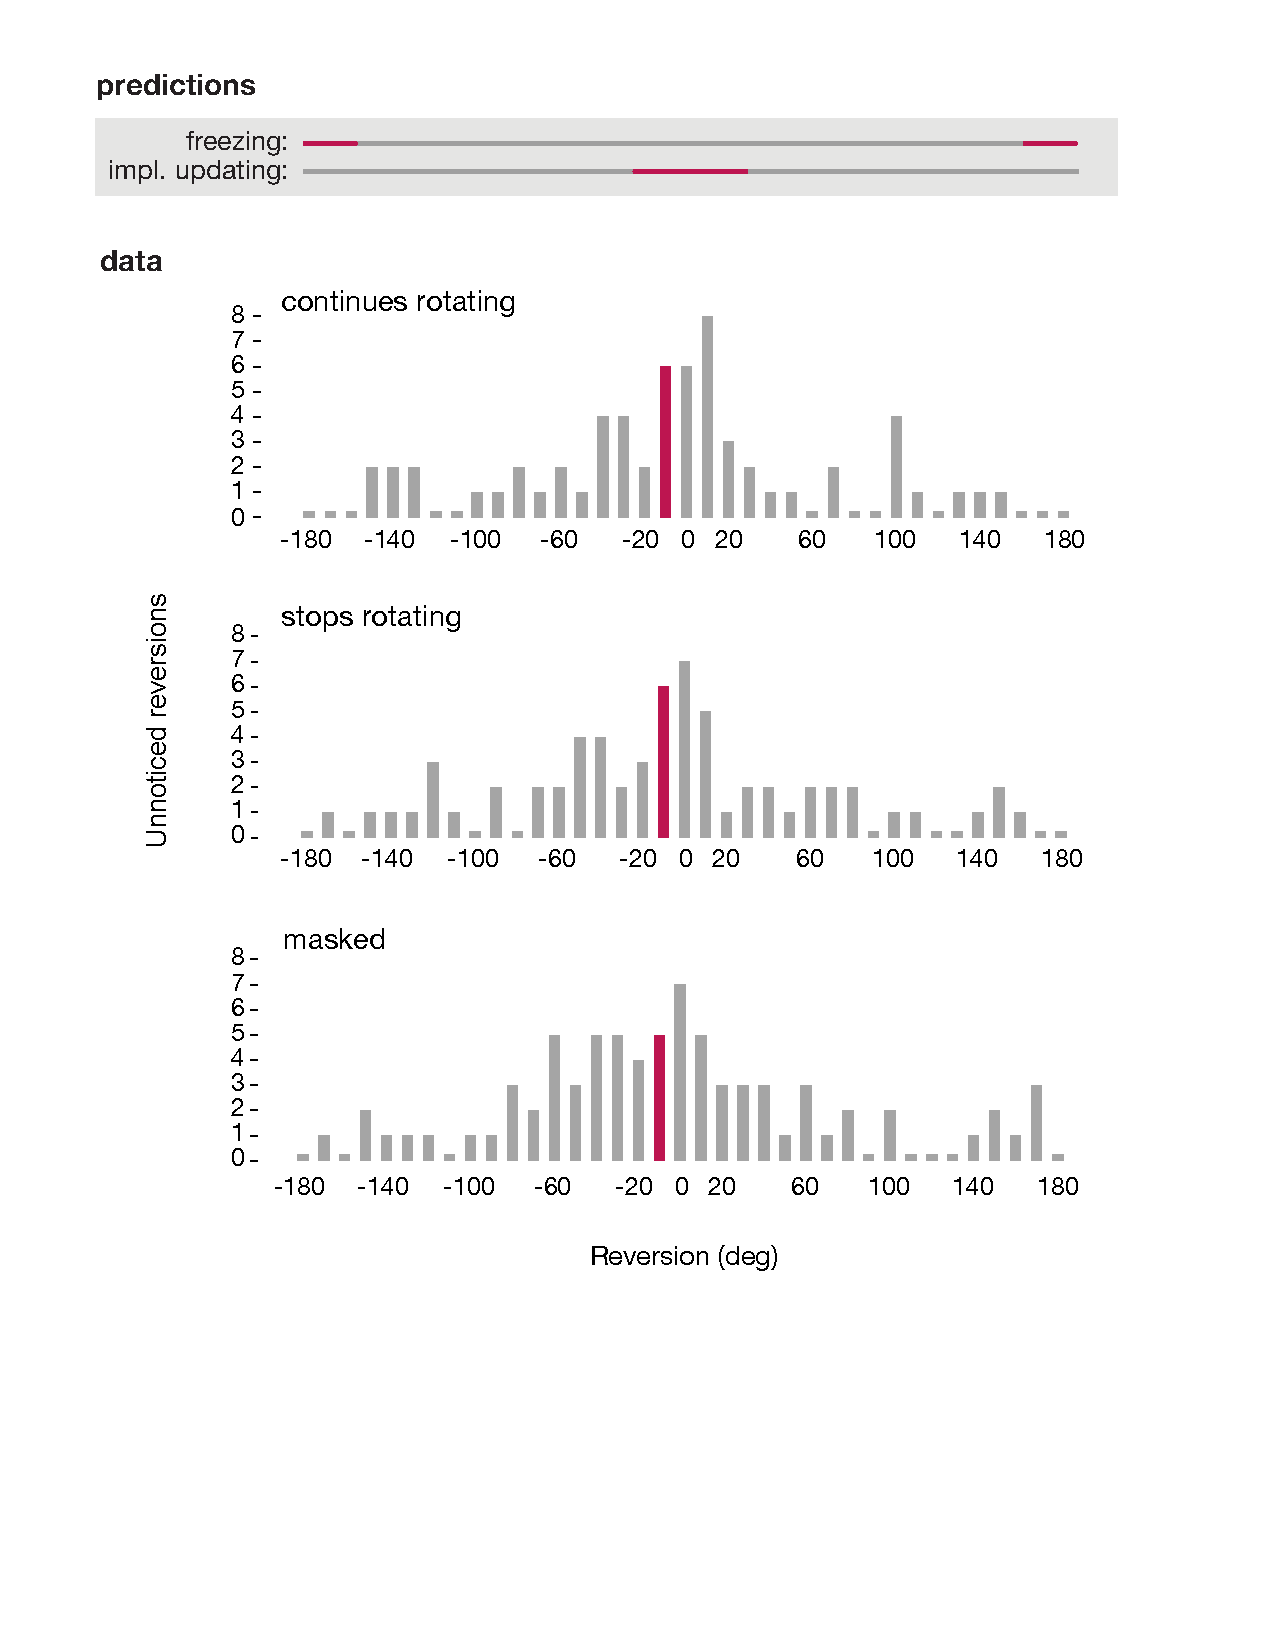
\includegraphics[width=4in]{figures/fig2.pdf}
\caption{Three histograms are shown. Note that...}
\label{fig:label1}
\end{center}
\end{figure}
